\section{Recent Phase-2 Results (5 Victims, 1 Attacker)}
This section reports the latest high-density multi-tenant experiment from \texttt{phase2\_5v1\_metrics.csv}. The test compares only two data-plane strategies under increasing attacker pressure:
\begin{enumerate}
  \item \textbf{Sidecar Isolation (Separate eBPF)}
  \item \textbf{Sidecarless Contention (Shared eBPF)}
\end{enumerate}

\subsection{Experimental Coverage}
The run matrix contains five attacker target levels and three repetitions per level for each configuration:
\begin{itemize}
  \item Noise targets: $\{0, 10{,}000, 20{,}000, 40{,}000, 60{,}000\}$ RPS
  \item Repetitions per (config, noise): $n=3$
  \item Total samples: $30$ rows ($15$ per configuration)
\end{itemize}

\subsection{Aggregate Means Across All Phase-2 Samples}
Across all noise levels and repetitions, the averaged metrics are:
\begin{itemize}
  \item \textbf{Sidecar Isolation}: $p50=1.483$ ms, $p95=4.436$ ms, $p99=8.090$ ms, throughput $=906.456$ QPS.
  \item \textbf{Sidecarless Contention}: $p50=1.522$ ms, $p95=4.643$ ms, $p99=8.547$ ms, throughput $=896.845$ QPS.
\end{itemize}

At aggregate level, sidecarless shows slightly higher tail latency and slightly lower throughput.

\subsection{Noise-Level Comparison}
The strongest separation appears at \textbf{20,000 RPS} attacker target:
\begin{itemize}
  \item Sidecar Isolation: mean $p99=9.078$ ms, throughput $=885.315$ QPS.
  \item Sidecarless Contention: mean $p99=11.930$ ms, throughput $=836.492$ QPS.
\end{itemize}

This corresponds to:
\begin{itemize}
  \item $\frac{11.930}{9.078} \approx 1.314\times$ higher $p99$ in sidecarless,
  \item $\frac{836.492}{885.315} \approx 0.945$ throughput ratio (about $5.5\%$ lower) in sidecarless.
\end{itemize}

At higher target rates (40k--60k RPS), both configurations show elevated latency and reduced throughput, while their relative ordering becomes less stable across repetitions.

\subsection{Figure for the Recent Run}
\begin{figure}[H]
  \centering
  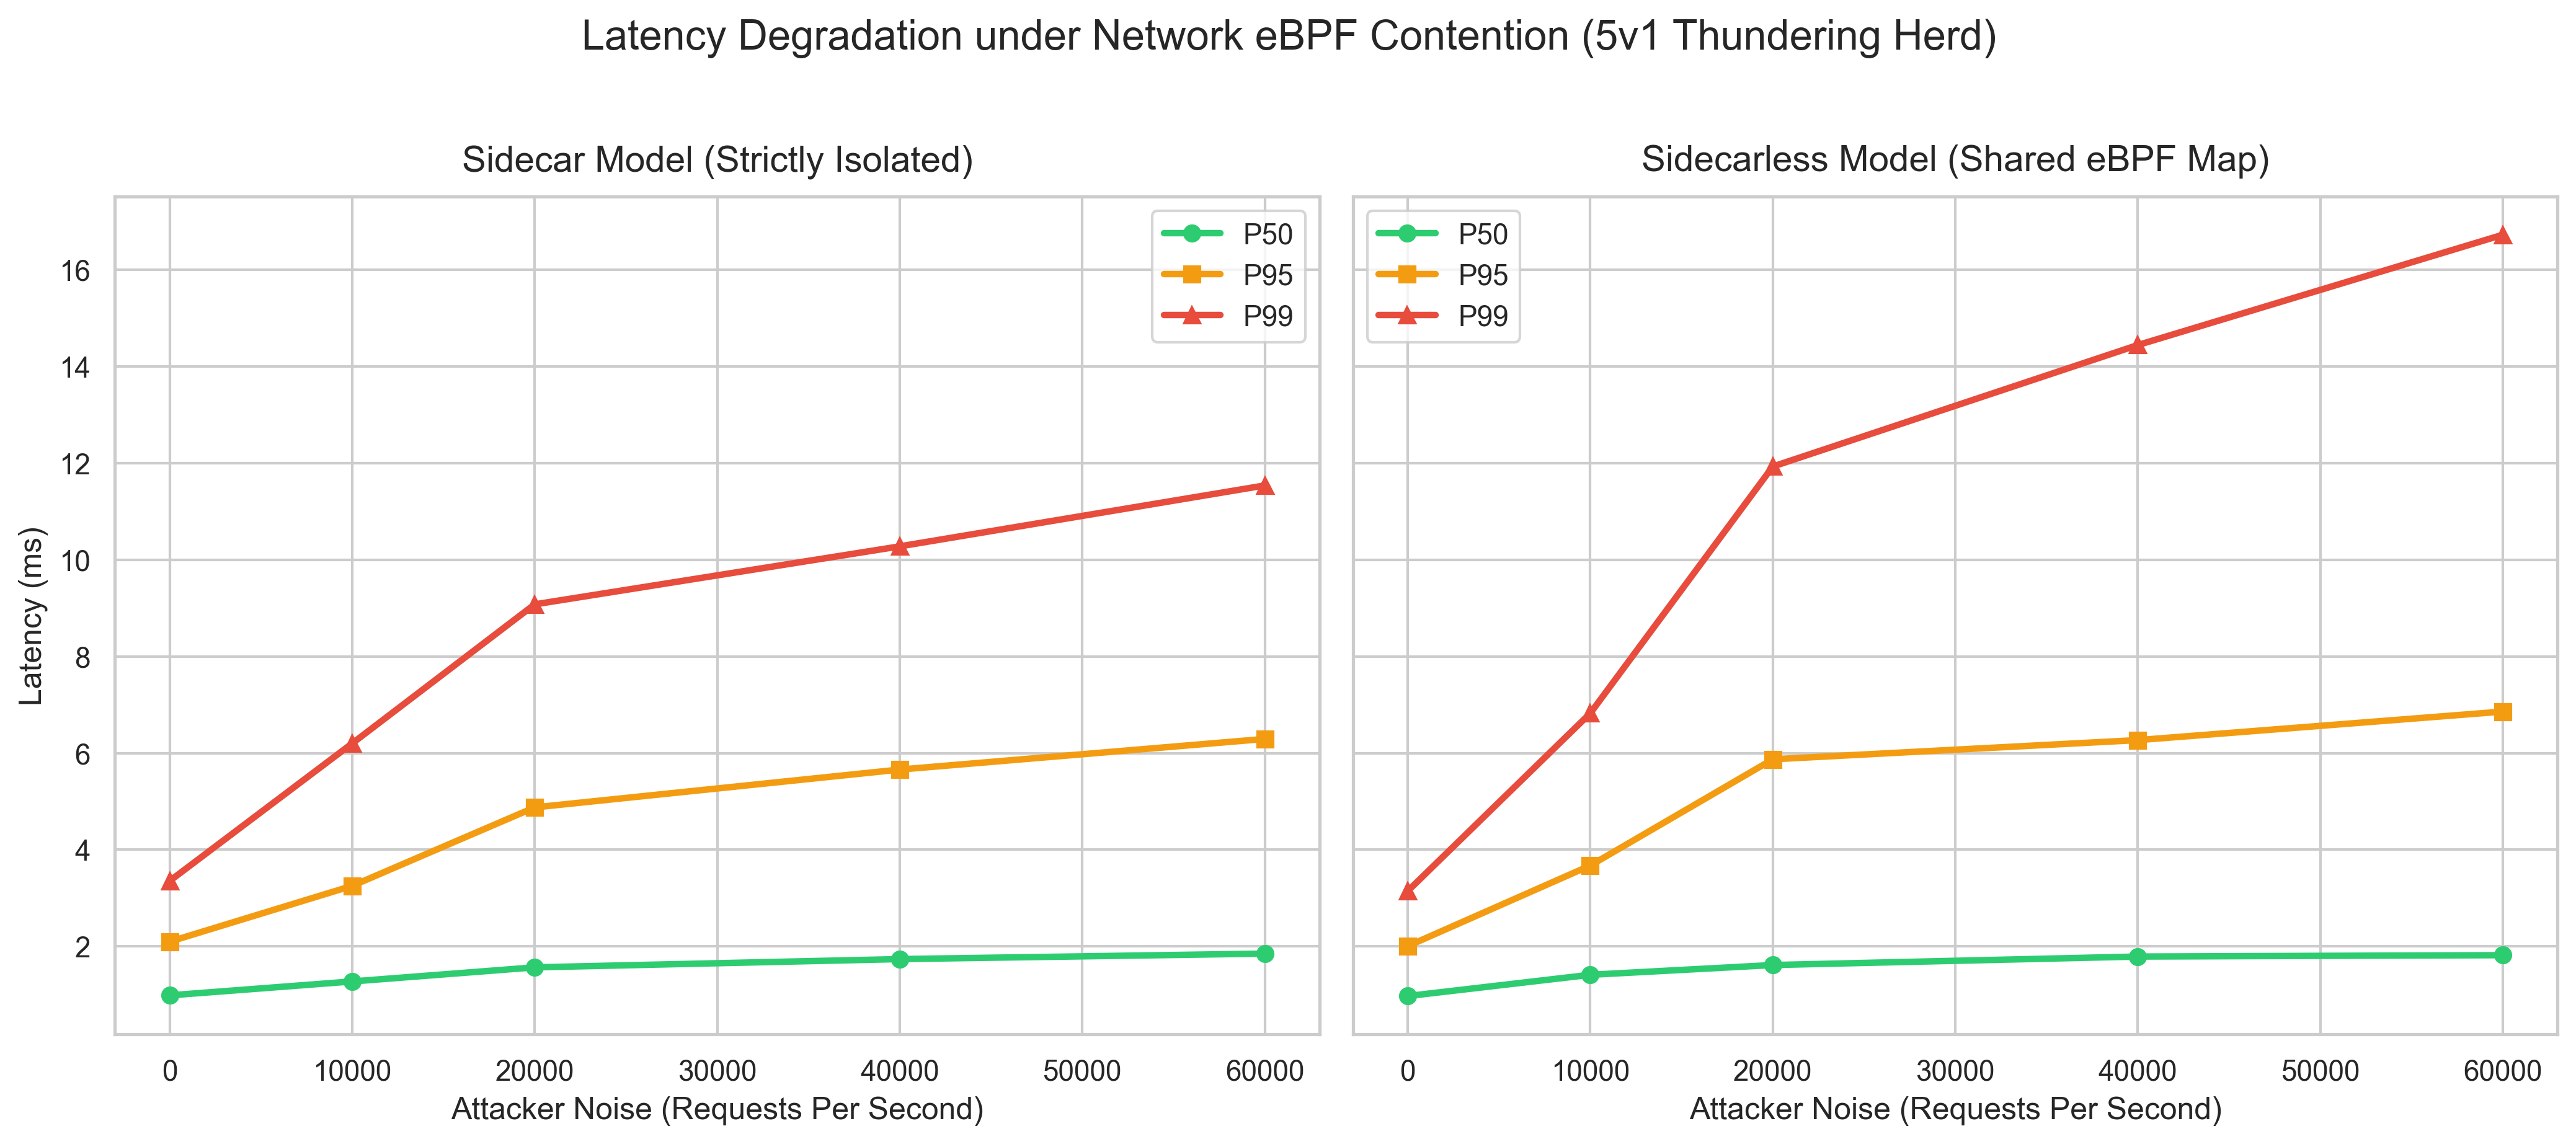
\includegraphics[width=0.95\linewidth]{../graphs/latency_degradation_chart.png}
  \caption{Recent Phase-2 (5v1) latency behavior under increasing attacker load for sidecar isolation and sidecarless contention.}
  \label{fig:phase2-5v1-latency}
\end{figure}

\subsection{Interpretation}
The recent 5-victim campaign shows that attacker pressure increases tail latency in both configurations. The most pronounced penalty for the sidecarless shared path occurs at the mid-high contention point (20k RPS), where both $p99$ inflation and throughput loss are visible relative to sidecar isolation. This supports the central observation that shared-path contention can amplify tail behavior under multi-tenant load.

